\documentclass{etit-workshop-protokoll}

%\kursnummer{0}
%\kurstitel{Leitfaden und Vorlage zur Ausarbeitung}

\kursnummer{1}
\kurstitel{Messwerterfassung und regenerative Energieerzeugung}

%\kursnummer{2}
%\kurstitel{Analoge Filter und Schaltungsanalyse}

%\kursnummer{3}
%\kurstitel{Sensorik}

%\kursnummer{4}
%\kurstitel{Digitale Signalverarbeitung}


\gruppennummer{116}

\teilnehmer{Jailan}{Oweda}{2257347}{ujzpo}{ujzpo@student.kit.edu}
\teilnehmer{MainAnh}{Vu}{2217409}{uxgce}{uxgce@student.kit.edu}
\teilnehmer{Andreas}{Tsouchlos}{2238886}{uhhxt}{uhhxt@student.kit.edu}

\renewcommand\thesubsubsection{\alph{subsubsection}}
\usepackage{gensymb}
\usepackage{graphicx}
\usepackage{circuitikz}

\begin{document}

\maketitle

\pagestyle{empty}% % leere Kopfzeile

\begin{abstract}
\section*{Abstract}
    \par In diesem Dokument werden die Ergebnisse der Bearbeitung des ersten Kurses des Workshops Elektro-
    und Informationstechnik wiedergeben und diskutiert. Hierbei handelt es sich um die Energiegewinnung
    mittels einer Solarzelle und der Zwischenspeicherung dieser Energie.
    Ziel dieser Arbeit ist die Untersuchung und Vermessung einer Solarzelle. Als erstes wird dafür die I-U-
    Kennlinie und die daraus ableitbare Leistung bestimmt. Danach wird an die Schaltung ein Kondensator
    angeschlossen. Sein Verhalten wird beim Laden sowie Entladen beobachtet und analysiert. Zuletzt wird
    das Verhalten des gesamten Aufbaus betrachtet.
    \par Zur Ausführung dieses Projekts werden eine Solarzelle, verschiedene Lichtquellen , das TI-Board als A/D-
    Wandler und Messgerät, ein Speicherkondensator sowie weitere elektronische Komponenten (z.B.
    Wiederstände und Dioden) verwendet.
    \par Zum Einarbeiten in die Thematik und um die Funktionsweise einiger Bauteile nachzuvollziehen, wurden Literaturen herangezogen. Für das Arbeiten mit den Messwerten wurde darüber hinaus die Software MATLAB des Unternehmens MathWorks eingesetzt. 
    \par Grundsätzlich kommt man zur Schlussfolgerung, dass die Leistungen in Abhängigkeit von der
    Beleuchtung variieren, dass die gemessenen Spannungen der Solarzelle unter den natürlichen
    Bedingungen von vielen Faktoren abhängen und abschließend dass Kondensatoren als Energiespeicher
    dienen, jedoch nicht optimal sind. Anschließend werden der Verlauf und die Resultate des Workshops in Latex dokumentiert.
\end{abstract}



\clearpage % neue Seite beginnen
\pagestyle{scrheadings} % Kopfzeilen zuruecksetzen

\tableofcontents
\listoffigures
\listoftables
\clearpage % neue Seite beginnen

\section{Einleitung}
    \par Nachhaltigkeit und Zukunftsfähigkeit bei der Energiegewinnung nehmen heutzutage an Bedeutung immer mehr zu. Hierbei spielt besonders regenerative Energieerzeugung eine immer größer werdende Rolle, vor allem auch hinsichtlich der Umweltbelastung herkömmlicher Energieerzeugungsmethoden. Unter regenerative Energieerzeugung fallen unter anderem Windenergie, Wasserkraft, Geothermie und Photovoltaik, welche alle auf die Solarstrahlung basieren. Dabei hat in den letzen Jahren die Bedeutung der Photovoltaik, die als einzige direkt die Solarenergie in elektrische Energie umwandelt, immer weiter zugenommen.
\par Erneuerbare Energiequellen sind aufgrund vieler Aspekte attraktiv. Bereits der Name impliziert, dass deren Energien nahezu unbegrenzt zur Verfügung stehen. Für die Nachhaltigkeit ist auch gesorgt, da die Energieerzeugung ohne Emissionen erfolgt und damit weit weniger umweltbelastend ist als herkömmliche Methoden. Es entstehen keine Kosten für jegliche Brennstoffe, im Gegensatz z.B zur Kohleenergie. Dazu kommt, dass die Energiequelle grundsätzlich vom Standort unabhängig ist, weshalb auch Entwicklungsländer in der Lage sind, ihre eigene Energie zu produzieren.
\par Allerdings handelt es sich bei regenerativer Energieerzeugung noch um eine relativ neue Technologie, weshalb sie wirtschaftlich in vielen Faktoren mit herkömmlichen Energieerzeugungsverfahren nicht mithalten kann. So ist der Ertrag im Gegensatz z.B zu dem von Kohle sehr gering, weshalb mit großen Investitionen gerechnet werden muss, wenn herkömmliche durch regenerative Quellen ersetzt werden sollen. Die hohen Kosten, die dadurch entstehen, machen sie wirtschaftlich unattraktiv. Da die regenerative Erzeugung von Energie stark vom Umfeld der Anlagen hinsichtlich der Umweltfaktoren abhängt, die diese produzieren, kommen weitere Kosten auf, um die Bevölkerung zuverlässig mit Energie versorgen zu können.
\par Im Vergleich zur Windenergie, Wasserkraft oder Geothermie, die indirekt durch Solarenergie angetrieben werden, wandelt Photovoltaik Solarenergie direkt in elektrische Energie um. Hierzu nutzt sie den photovoltaischen und den photoelektrischen Effekt: Solarstrahlung trifft auf die Oberfläche einer Solarzelle. Dadurch werden manche Elektronen der äußeren Schichten der Atome der Solarzelle angeregt und fließen vom Valenzband ins sogenannte Leitungsband. Eine spezielle Bearbeitung des Materials verhindert, dass die Elektronen das Leitungsband wieder verlassen. Dadurch entsteht auf der einen Seite der Solarzelle ein Elektronenüberschuss und auf der anderen Seite ein Mangel, was anschließend zu einem Strom führt.
\par Die I-U-Kennlinie beschreibt die Stromstärke in Abhängigkeit der Spannung. So gibt der Flächeninhalt dieser die Leistung wieder. Ist die Fläche unter dem Graphen maximal, handelt es sich um den Maximum Power Point: Dem Punkt, an dem die Solarzelle mit maximaler Leistung arbeitet.
\par Eine Möglichkeit zur Energiespeicherung ist es, eine Energieart in eine andere umzuwandeln. Mehrmalige Umwandlungen sind zwar mit Energieverlust verbunden, haben im Vergleich zur direkten Energiespeicherung, z.B durch Kondensatoren, verschiedene Vorteile. Allgemein betrachtet hat jede Form der Energiespeicherung ihre Stärken und Schwächen, weshalb je nach Situation andere Methoden benutzt werden müssen. Durch weitere Forschung in diesem Gebiet, kann jedoch die Effizienz vieler dieser Methoden verbessert werden.

% Frühere Version

%\par Nachhaltigkeit und Zukunftsfähigkeit bei der Energiegewinnung nehmen heutzutage an Bedeutung
%zu. Hierbei spielen besonders regenerative Energieerzeugung eine immer größer werdende Rolle
%hinsichtlich des Umweltsaspekts. Unter regenerativer Energieerzeugung fallen unter anderem
%Windenergie, Wasserkraft, Geothermie und Photovoltaik, welche alle auf die Solarstrahlung
%basieren. (vgl. S.31 Photovoltaik). Dabei hat in den letzten zehn Jahren die Bedeutung der
%Photovoltaik, welche die Solarstrahlung direkt in elektrische Energie umwandelt, immer stärker
%zugenommen (vgl. S. 7, Erneuerbare Energien in Deutschland
%$https://www.umweltbundesamt.de/sites/default/files/medien/376/publikationen/180315_uba_hg_
%eeinzahlen_2018_bf.pdf)$
%\par Erneuerbare Energien wirken aufgrund vieler Aspekte attraktiv. So impliziert bereits der Name, dass
%die Energiequellen nahezu unbegrenzt zu Verfügung stehen. Für eine nachhaltige Zukunft ist es
%ebenso vorteilhaft, dass dessen Energieerzeugung ohne Emissionen erfolgt. Infolgedessen tauchen
%keine schwerwiegenden Konsequenzen und Bedrohungen für die Umwelt auf. Im Gegensatz zu
%Kohleenergie entstehen keine Kosten für jegliche Brennstoffe. Dazu kommt, dass die Energiequelle
%nicht komplett abhängig vom Standort ist und somit überall nutzbar ist, weshalb auch
%Entwicklungsländer in der Lage sind, selber Energie zu produzieren.
%\par Allerdings handelt es sich bei regenerativer Energie noch um eine neue Art der Energieerzeugung,
%sodass sie wirtschaftlich in vielerlei Dingen nicht effektiv ist im Vergleich zu der bisherigen
%herkömmlichen Energieerzeugung. So ist die Energiedichte im Gegensatz zu der von beispielsweise
%Kohle sehr gering, weshalb mit Quantität entgegengewirkt werden muss. Dieser hohe
%Materialverbrauch ist ein weiterer negativer Aspekt. Zudem entstehen somit hohe Kosten, wenn
%man in erneuerbare Energien investieren will, was diese wirtschaftlich unattraktiv macht. So muss
%man auch das Argument der Unerschöpflichkeit relativieren, da das Energieangebot stark variiert. So
%ist der Energieertrag insbesondere bei Photovoltaik und Windkraft von Umweltfaktoren abhängig.
%Aufgrund dessen kann der Energiebedarf der Bevölkerung nur zuverlässig abgedeckt werden, indem
%die Anzahl der Kraftwerke erhöht wird, was wiederum mit hohen Kosten verbunden ist.
%Photovoltaik wandelt elektrische Energie direkt um, indem die den photovoltaischen Effekt nutzt.
%Diese lässt sich an einem Halbleiter erläutern. Lichtwellen treffen auf die eine Oberfläche und geben
%ihre Energie an Elektronen ab, welche aus ihrer Verbindung sich lösen und aufgrund der Dotierung in
%Richtung des Pluspols wandern. Auf der anderen Seite des Kabels kommen Elektronen nach, welche
%die Löcher füllen. Die ladungsfreie Zone wird überbrückt.
%\par Die I-U-Kennlinie beschreibt grafisch die Stromstärke in Abhängigkeit der Spannung. So ergibt der
%Flächeninhalt dieser die Leistung wieder. Ist diese Fläche unter dem Graphen maximal, handelt es
%sich um den Maximum Power Point, welche den Punkt markiert, an der die Solarzelle mit maximaler
%Leistung arbeitet.
%\par Eine Möglichkeit zu Speicherungen ist es, diese Energien in andere Energiearten umzuwandeln. Diese
%mehrmaligen Umwandlungen sind zwar mit Energieverlust verbunden, jedoch sind sie immer noch
%effizienter als die direkte Energiespeicherung mit Speicherkondensatoren. Allgemein lässt sich sagen,
%dass die Speichermöglichkeiten alle ihre Schwächen haben und an ihnen noch weitergeforscht
%vwerden muss, damit die Effizienz gesteigert wird.

\section{Aufgaben}
    \subsection {Literaturrecherche}                                    % 2.1
    ABCD

    \subsection {Vermessung der Solarzelle POW112D2P}                   % 2.2
    \subsubsection{Aufnehmen der I-U Kennlinie}                         % 2.2 a
        \textbf{Methode}
        \newline
        
        \par Zunächst soll die Solarzelle mit drei unterschiedlichen Lichtquellen bestrahlt werden. 
        Für die Messung kommen folgende Bauteile zum Einsatz, wobei der Speicherkondensator erst in den angehenden Aufgaben verwendet wird.
        \begin{table}[H]
        	\centering
        	\caption{Verwendetes Material}
        	\label{tab:Bauteile}
        	\begin{tabular}{ccc}
        		\toprule
        		Bauteiltyp & Bezeichnung / Beschreibung & Wert\\
        		\midrule
        		Solarzelle & SEEED Studio POW112D2P  & U\textsubscript{OC} = 5,5V, I\textsubscript{SC} = 4 mA bei 5 klx \\
        		Zener-Diode & ZF 5,1; 5,1V 0,5W  & V = 5,1 V; P = 0,5W \\
        		Speicherkondensator & Panasonic 5,5V 220 mF & V = 5,5V; C = 220,0mF \\
        		Stützkondensator & Keramikkondensator Code 104 & C = 100,0nF \\
        		Widerstand & Kohleschichtewiderstände  & 10$\Omega$ - 10M$\Omega$ ; P = 0,25W; 5\% \\
        		Steckbrett & Breadboard
        		& \ \\
        		Drahtbrücke & Drahtbrücken-Set 140-teilig
        		& \ \\
        		\bottomrule
        	\end{tabular}
        \end{table}
    	\vspace{1mm}
        Hierbei wird eine Schaltung aufgestellt, bestehend aus einer Diode, welche eine umgekehrte Stromrichtung verhindert, einer Zener-Diode, die die maximale Spannung eingrenzt, und einem Spannungsteiler. Angeschlossen werden die Solarzelle sowie das TI-Board. Diese ist in Abbildung \ref{fig:Schaltkreis} dargestellt.
        \begin{figure}[H]
            $$
            \ctikzset{bipoles/length=1cm}
            \begin{circuitikz}[european] \draw
                (0,0) to[current source, l={\footnotesize $\small Solarzelle$}] (0,4)
                (0,4) to[stroke diode, l={\footnotesize $Diode$}] (2,4)
                (2,0) to[stroke Zener diode, l_={\footnotesize $Zener\ Diode$}] (2,4)
                (0,0) to (2,0)
                (2,4) to (6,4)
                (6,4) to[R, l={\footnotesize $100\ k\Omega$}] (6,2)
                (6,2) to (5,2)
                (5,2) to[capacitor, l_={\footnotesize $100\ nF$}] (5,0)
                (2,0) to (5,0)
                (6,2) to[R, l={\footnotesize $100\ k\Omega$}] (6,0)
                (5,0) to (6,0)
                (6,2) to (8,2)
                (8,2) to[voltmeter, o-o] (8,0)
                (6,0) to (8,0)
                (6,4) to (10,4)
                (10,4) to[R, o-o, l={\footnotesize $Variabler\ Widerstand$}] (10,0)
                (8,0) to (10,0)
                ;
            \end{circuitikz}
            $$
            
            \caption{Benutzter Schaltkreis}
            \label{fig:Schaltkreis}
        \end{figure}
        
        \par Unter gleichbleibenden Bedingungen wurde die Spannung in Abhängigkeit des Widerstandes gemessen, indem Widerstände in Reihe geschaltet wurden. Es wurden in diesem Fall zwölf Widerstände in einem Intervall zwischen 10$\Omega$ bis 5200$\Omega$ verwendet. Mit MatLab lässt sich die Stromstärke aufgrund von I = U/R ermitteln, sodass man sich den Graphen der Stromstärke in Abhängigkeit der Spannung zeichnen lassen kann. (vgl. S.18, \cite{kalman})
        Die Werte der Lichtquellen sind in Tabelle \ref{tab:Werte} abgebildet:
        \begin{table}[H]
        	\centering
        	\caption{Angaben über Lichtquellen}
        	\label{tab:Werte}
        	\begin{tabular}{ccc}
        		\toprule
        		Art & Leistung & Abstand \\
        		\midrule
        		Halogenlampe & 500W  & 70cm \\
        		Leuchtstoffröhre & 24W  & 13cm \\
        		LED & 40W & 2,5cm \\
        		\bottomrule
        	\end{tabular}
        \end{table}
        
        \vspace{5mm}
        \textbf{Ergebnis}
        \newline
        
        \begin{figure}[H]
            %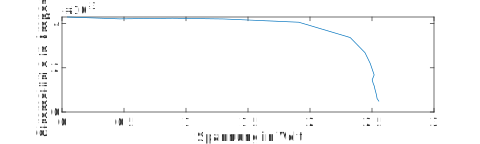
\includegraphics{spannung_halogen}
            \def\svgwidth{\textwidth}
            \input{spannung_halogen.pdf_tex}
            
            \caption{Stromstärke in Abhänigkeit der Spannung bei der Halogenlampe}
        \end{figure}
        
        \begin{figure}[H]
            %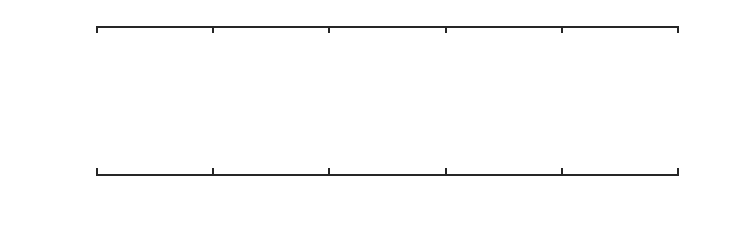
\includegraphics{spannung_lsr}
            \def\svgwidth{\textwidth}
            \input{spannung_lsr.pdf_tex}
            
            \caption{Stromstärke in Abhänigkeit der Spannung bei der Leuchtstoffröhre}
        \end{figure}
        
        \begin{figure}[H]
            %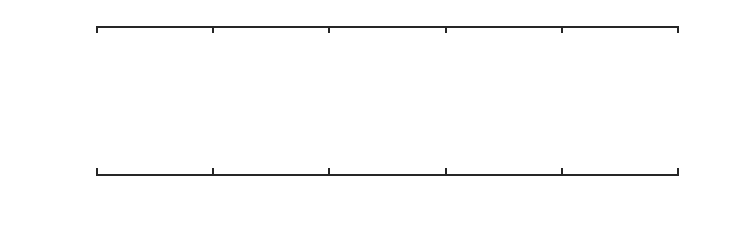
\includegraphics{spannung_led}
            \def\svgwidth{\textwidth}
            \input{spannung_led.pdf_tex}
            
            \caption{Stromstärke in Abhänigkeit der Spannung bei der LED}
        \end{figure}

    \subsubsection{Bestimmung des Maximum-Power-Points (MPP)}           % 2.2 b
        \textbf{Methode}
        \newline
        \par Die Leistung hängt von der Spannung sowie der Stromstärke ab aufgrund des Zusammenhanges $P=U*I$ (vgl. S.28, LEN Skript). Alternativ gilt wegen $I=U/R$ ebenfalls $P=U^2/R$, welche hier bevorzugt wird, da die Spannung sowie der Widerstand direkte Messwerte sind. Das vorhandene Skript für die Ermittlung der Stromstärke wird um einen Vektor für die Leistung erweitert.
        Der Maximum Power Point (wird nun MPP abgekürzt) bezeichnet nun den Punkt, an dem die Leistung am größten ist (vgl. S.99f., Photovoltaik). Dieser maximale Wert für die Leistung sowie der dementsprechende Widerstand lassen sich ablesen oder von MatLab ausgeben. 
        
        \vspace{4mm}
        \noindent
        \textbf{Ergebnis}
   
        Die Werte der MPPs für unsere Lichtquellen betragen:
        \begin{table}[H]
        	\centering
        	\caption{MPPs der Solarzelle mittels verschiedener Lichtquellen}
        	\label{tab:MPP}
        	\begin{tabular}{ccc}
        		\toprule
        		Art & maximale Leistungsabgabe & Widerstand \\
        		\midrule
        		Halogenlampe & 0,0313W  & 690$\Omega$ \\
        		Leuchtstoffröhre & 0,0075W  & 1720$\Omega$ \\
        		LED & 0,0059W & 2200$\Omega$ \\
        		\bottomrule
        	\end{tabular}
        \end{table}
    
		%Absatz fällt wegen Tabelle weg    
        %\par Der MPP der Solarzelle unter der Verwendung einer Halogenlampe beträgt ca. 0,0313W und tritt bei %690 Ohm auf. Mit einer Leuchtstoffröhre liegt die maximale Leistung bei ungefähr 0,0075W, welche bei %einem Widerstand von 1720 Ohm erreicht wird. Wird hingegen eine LED als Lichtquelle eingesetzt, befindet %sich der MPP bei ca. 0,0059W bei einem Widerstand von 2200 Ohm.
        \par Anzumerken ist, dass es sich hierbei nur um grobe Näherungswerte für die maximale Leistung handelt, da lediglich zwölf Messwerte für die Leitung vorliegen. Für eine genauere Bestimmung des MPPs kann mithilfe dieser Werte eine Näherungsfunktion aufgestellt werden, mit dessen Ableitung das Maximum ermittelt werden kann. 
        Diskussion:
        \par Eine weitere Methode zur Bestimmung des MPPs ist über die Spannung und die Stromstärke möglich. So ist die Leistung das Produkt dieser, was auf die I-U-Kennlinie bezogen bedeutet, dass die Leistung den Flächeninhalt unter einem Punkt des Graphen widerspiegelt. So bezeichnet man den Punkt der Kennlinie als MPP, unter dem die Fläche U*I am größten ist. (vgl. S.99, Photovoltaik)
        \par Dieser Zusammenhang wird in dem folgenden Diagramm veranschaulicht.
        \par (Diagramm mit MPP fehlt)

    \subsubsection{MPP-Anpassung}                                       % 2.2 c
        \textbf{Diskussion}
        \newline
        \par Solarwechselrichter sind dafür zuständig, die von der Solarzelle produzierte Gleichspannung in Wechselspannung umzuwandeln. Für die maximale Leistungsausbeute bildet der im Solarwechselrichter enthaltende MPP-Tracker den optimalen Widerstand für den MPP, welcher jedoch unter natürlichen Bedingungen von verschiedenen äußeren Faktoren wie Verschattung, Temperatur oder Lichteinfall abhängt, sodass der MPP stets neu ermittelt werden muss (vgl. S.8f, Diplomarbeit). 
        
        \par Vernachlässigt wurden Diode/Zehnerdiode, da dort auch Spannung noch abfallen, kleiner Messfehler.

    \subsection {Langzeitmessung}                                       % 2.3
    \subsubsection{Spannungsverlauf und Leistung}                       % 2.3 a
        \textbf{Methode}
        \newline
        \par 
    
    
    
    
    
        Folgende Graphen zeigen den Verlauf der Spannung und der Leistung in abhänigeit der Zeit. Gemessen wurde am 5.10.2018 im Forum des KIT - Campus zwischen 11:30 Uhr und 13:30 Uhr, mit leichter bewölkung und einer Temperatur zwischen $10^{\circ}C$ und $15^{\circ}C$
        \begin{figure}[H]
            %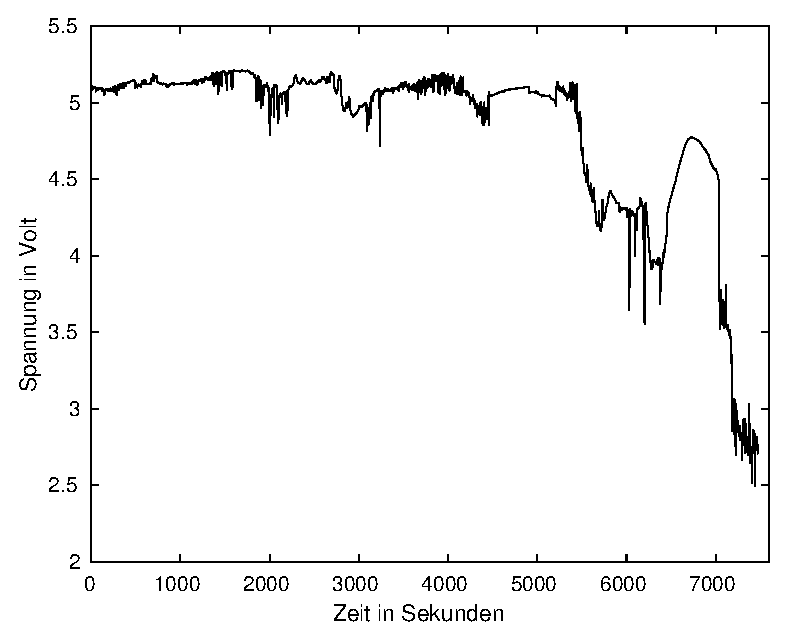
\includegraphics{spannung_langzeit}
            \def\svgwidth{\textwidth}
            \input{spannung_langzeit.pdf_tex}
            
            \caption{Spannungsverlauf über 2 Stunden}
        \end{figure}

        \begin{figure}[H]
            %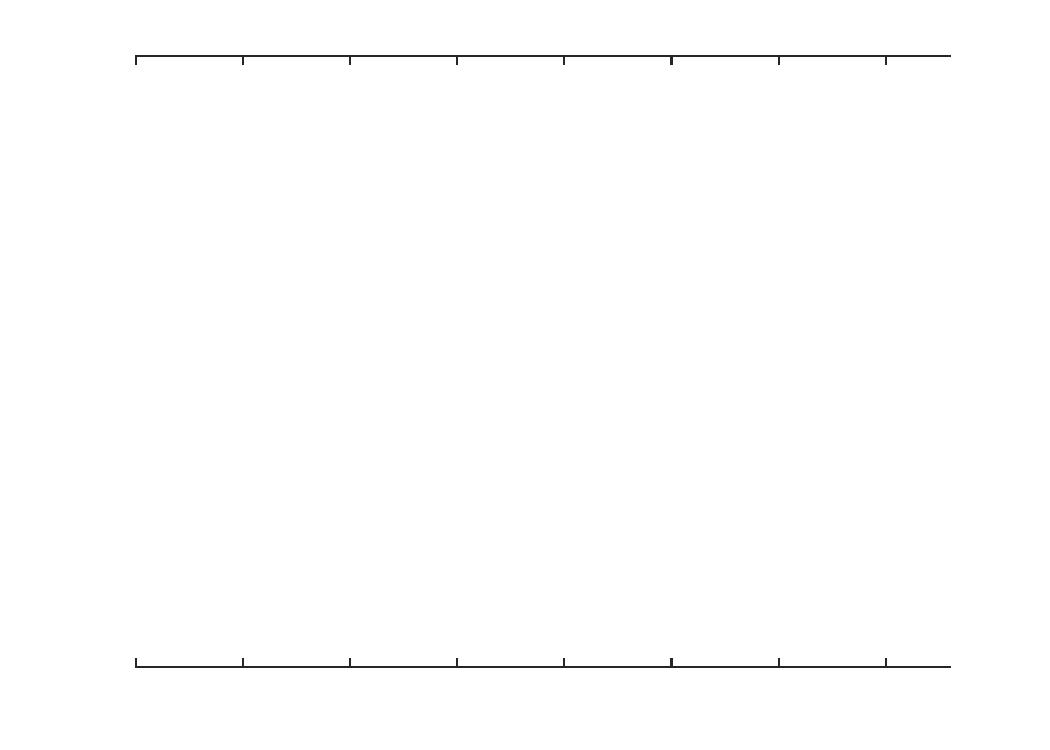
\includegraphics{leistung_langzeit}
            \def\svgwidth{\textwidth}
            \input{leistung_langzeit.pdf_tex}
            
            \caption{Leistungsverlauf über 2 Stunden}
        \end{figure}
        
        Die erzeugte Energie beträgt ungefähr 177.34 Ws bzw. 0.0237 Wh.

        
        
        
        
        
    \subsubsection{Energiegewinnung}                                    % 2.3 b
        \par Die Energiegewinnung mit Solarzellen wird von vielen Faktoren beeinflusst, die von der Umwelt der Solarzelle, aber auch von ader Zelle selbst abhängen.
        \begin{itemize}
            \item Der Winkel in dem die Strahlung auf die Solarzelle eintrifft: Beträgt dieser genau $90^{\circ}$, so ist die Energiegewinnung maximal. Umso größer der Winkel ist, desto kleiner ist die Menge an Strahlung, die von der Solarzelle abgefangen wird.
            \item Die Temperatur: Bei wechselnder Temperatur bleibt die Spannung größtenteils unverändert. Doch je größer die Temperatur ist, desto kleiner wird die Stromstärke die von der Solarzelle ausgeht, und damit auch die Leistung und die Energie.
            \item Das Wetter bzw. Klima: Zum einen beeinflusst es den Einfallswinkel des Lichtes, zum Anderen die Intensität der Strahlung selbst, indem z.B Wolken die direkte Bestrahlung der Zelle verhindern. Die Energiegewinnung mit einer Solarzelle ist also auch Orts- bzw. Zeit-abhänging.
            \item Das Material aus dem die Solarzelle angefertigt wurde: Wird beispielsweise sogennantes monokristallines Silicium verwendet, ist der Wirkungsgrad besonders hoch, ungefähr 25\%. Wird polykristallines Silicium benutzt, fällt der Wirkungsgrad auf 18 - 20 \% und bei amorphem Silicium sind es 5 - 7 \%. 
        \end{itemize}

    \subsection {Energiespeicherung und Verhalten von Solarzellen}      % 2.4
    \subsubsection{Theoretische Betrachtung}                            % 2.4 a
        \textbf{Diskussion}
        \newline
        \par Ein Kondensator besteht aus zwei Metallflächen, die durch einen Isolator getrennt sind. Er dient zur Ladungsspeicherung, indem man ihn an eine Spannungsquelle schaltet. Die davor gleichmäßig verteilten Elektronen werden vom Minus-Pol gezogen, welches mit dem Plus-Pol der Quelle verbunden ist. Somit wird der Kondensator elektrisch geladen. Würde man jetzt die Spannungsquelle mit einem Widerstand wechseln, dann würde der Kondensator als Spannungsquelle fungieren und sich entladen. Der Minus-Pol des Kondensators, wo sich früher die Elektronen gelagert haben wird neutral, indem die Elektronen über dem Widerstand vom Plus-Pol weggezogen werden. Der Isolator sorgt dafür, dass der Minus- und Plus-Pol nie direkt in Verbindung kommen, so dass die Elektronen immer über einen Leiter wandern müssen.
        
        $$
            \tau = R * C = 500 \Omega * 220mF = 110s
        $$
        
    \subsubsection{Messung}                                             % 2.4 b
        \textbf{Methode/Materialien}
        \newline
        \par Hier soll an der bisherigen Schaltung ein Speicherkondensator (V =5,5 V; C =220,0 mF) angeschlossen
        werden. Unter konstanter Bestrahlung der Solarzelle wird die Spannung beim Aufladen des
        Kondensators gemessen. Als nächstes soll das Licht ausgeschaltet werden und der Kondensator soll mit
        einem 500 Ohm Widerstand angeschlossen werden, damit er sich entlädt.
        \vspace{4mm}
        \newline
        \textbf{Ergebnis}
        \newline
        \par
        \begin{figure}[H]
            %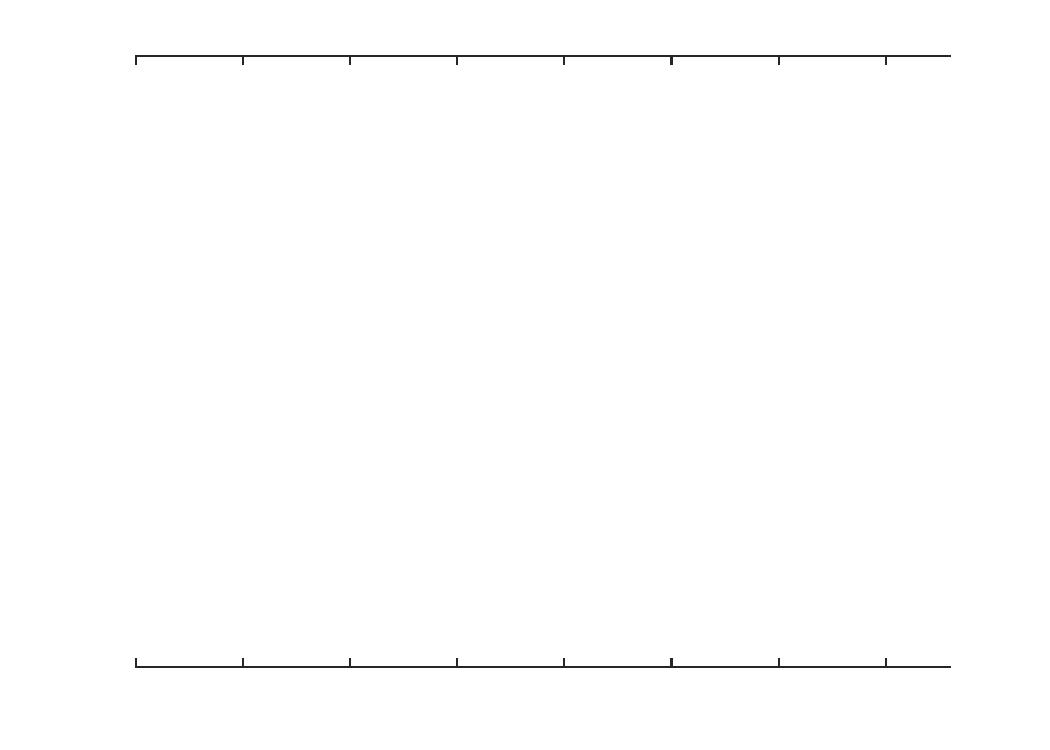
\includegraphics{leistung_langzeit}
            \def\svgwidth{\textwidth}
            \input{spannung_aufladen.pdf_tex}
            
            \caption{Spannungsverlauf bei Aufladen des Kondensators}
        \end{figure}
        \begin{figure}[H]
            %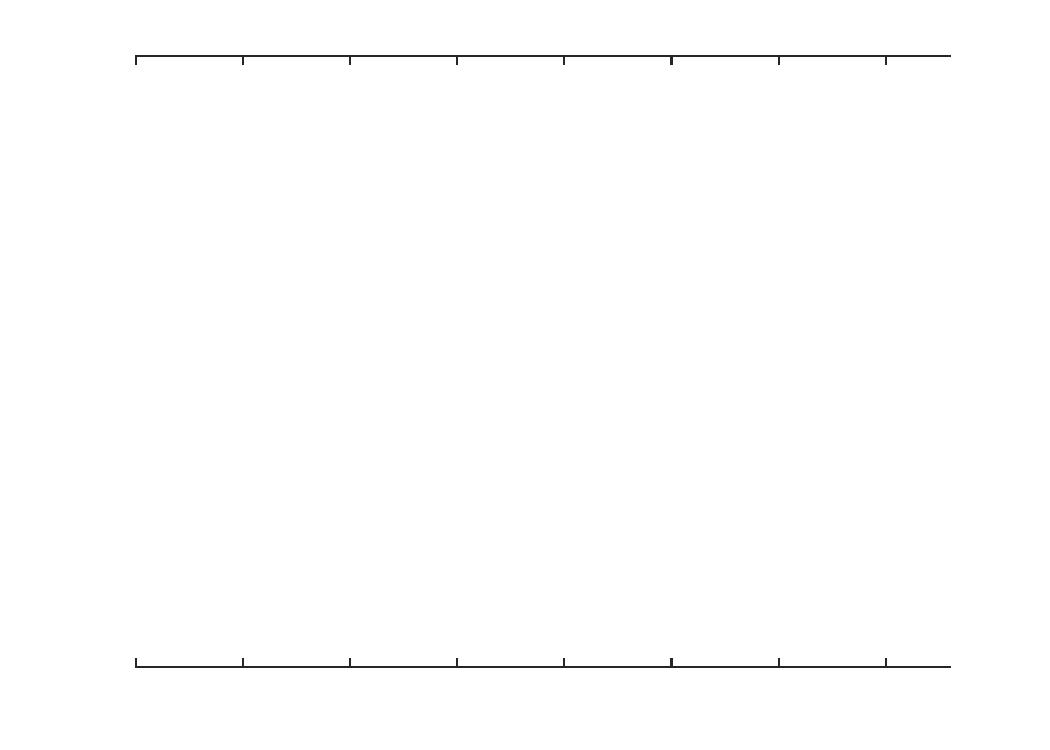
\includegraphics{leistung_langzeit}
            \def\svgwidth{\textwidth}
            \input{spannung_entladen.pdf_tex}
            
            \caption{Spannungsverlauf bei Entladen des Kondensators}
        \end{figure}
        
        \clearpage
    \subsubsection{Modellbildung}                                       % 2.4 c
        \textbf{Diskussion}
        \newline
        \par Die in der letzten Teilaufgabe gezeigten U-I-Diagramme sind hier zu vergleichen. Beim Aufladen sieht
        man, dass je größer die Spannung wird, umso mehr sich die Stromstärke den Wert Null annähert. Die
        Kurve fängt bei einem Wert von ungefähr 2.7mA an, wo noch fast keine Spannung fließt. Die
        Stromstärke sinkt rapide. Je näher sie sich der Null nähert, umso langsamer sinkt sie. Die Spannung
        dagegen steigt kontinuierlich, bis sie ihren Grenzwert bei ungefähr 0.42V erreicht. Beim Entladen sollte
        man den Graphen von rechts nach links lesen, weil die Spannung sinkt. Die Kurve fängt bei ca. -3.5mA
        und 0.36V an. Hier sind die Werte von der Stromstärke im negativen Bereich zu sehen. Wieder nähert
        sich die Stromstärke der Null an, aber diesmal indem sie steigt. Je kleiner die Spannung ist, umso größer
        wird die Stromstärke.
        \par Beim Aufladen eines Kondensators, steigt die Spannung bis zum Maximalwert. Dabei steigt auch der
        Widerstand des Kondensators, denn er kann ab einer bestimmten Spannung zerstört werden. Weil es
        weniger Elektronen gibt, die auf dem Pluspol des Kondensators sind, fließt weniger Strom durch. Wird
        der Maximalwert der Spannung erreicht, dann fließt kein Strom mehr. Der Widerstand des
        Kondensators wird dabei unendlich groß.
        \par Beim Entladevorgang wirkt der Kondensator wie eine Spannungsquelle mit einem sehr kleinen
        Innenwiderstand. Es fließt ein Strom in der entgegengesetzten Richtung, was erklärt, warum die
        Stromstärke im negativen Bereich liegt. Die Spannung sinkt vom Maximalwert auf Null und genauso
        sinkt die Stromstärke. Wenn der Kondensator entladen ist, dann fließt kein Strom mehr.
        Um die Solarzelle besser zu beschreiben, soll eine Stromquelle als Modell benutzt werden, denn die
        Stromstärke verändert sich im Verhältnis zur Spannung kaum.

        \clearpage
    \subsubsection{Gesamtenergie und Wirkungsgrad}                      % 2.4 d
        \textbf{Methode/Materialien}
        \newline
        \par
        \begin{figure}[H]
            \lstinputlisting[language=Matlab, frame=single, firstline=17]{messungen/Aufgabe_2_4/Energie.m}
            \caption{Matlab-Skrip zur Berechnung des Wirkungsgrades}
        \end{figure}
        \vspace{4mm}
        %\newline
        \textbf{Ergebnis}
        \newline
        \par Wirkungsgrad: 79.42\%
        \vspace{4mm}
        \newline
        \textbf{Diskussion}
        \newline
        \par Recherchen zeigen (Quelle aus Internet), dass der Wirkungsgrad unserer Messung um 10 % abweicht, da
        sie bei 90% liegen sollte. Diese Differenz kann auf mehrere Faktoren zurückgeführt werden.
        In der letzten Teilaufgabe ist zu sehen, dass das Aufladen des Kondensators bei ca. 0.42V aufhört und
        das Entladen bei ca. 0.36V anfängt. Dies bedeutet, dass zwischen den beiden Vorgängen Spannung
        verloren gegangen ist. (Speicherdauer)
        \par Außerdem könnten es Messfehler geben. Z.B. könnte der Raum beim Entladevorgang nicht dunkel
        genug gewesen sein, sodass die falschen Spannungen gemessen wurden. Darüber hinaus ist zu beachten, dass die Wärmeverluste immer mitgemessen wurden. (Einen Messfehler aufgrund von Wärmeverlust kann ausgeschlossen werden, da dieser sowohl bei der Aufladung als auch bei der Entladung bereits enthalten war).
        Auffällig sind zudem die Graphen beider Messungen. Die Werte schwanken relativ stark. Eine Begründung für diese Schwankungen können äußere Faktoren sein. So wurde die Messung in einem nicht vollständig abgedunkelten Raum durchgeführt. (Wie genau Einfluss?) Im Nachhinein hätte man, statt die Solarzelle abzudunkeln, diese abkoppeln können, sodass auch Restlicht keinen Einfluss hat. 
        Mittlerweile ist die Technik so weit weiterentwickelt, dass der Wirkungsgrad schon bei 97\% liegt (vgl. KIT PAPER) 

    \subsection {Verhalten Photovoltaik mit und ohne Energiespeicher}   % 2.5
    \subsubsection{Messung}                                             % 2.5 a
        \textbf{Methode}
        \newline
        \par Die Messungen werden wie in der Schaltskizze ausgeführt. Beim zweiten Durchlauf wird ein Kondensator parallelgeschaltet. Der Verlauf der Messkurven wird in der folgenden Abbildung abgebildet:
        
        \begin{figure}[H]
            %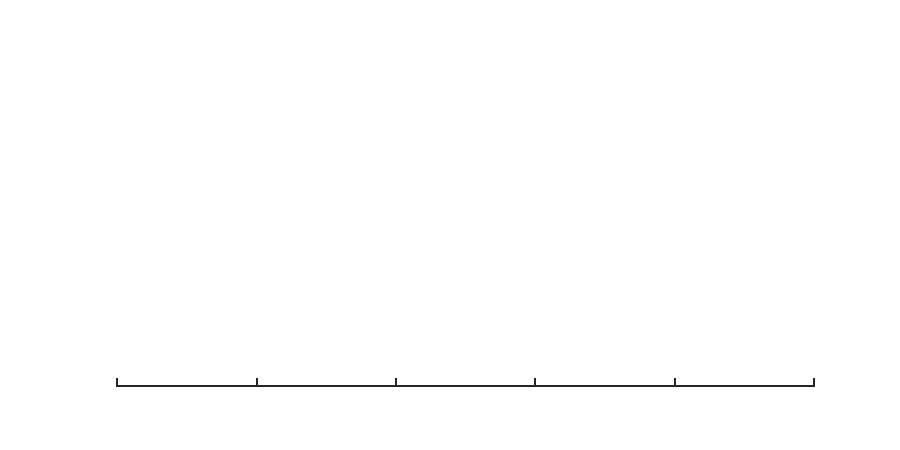
\includegraphics{spannung_kondensator}
            \def\svgwidth{\textwidth}
            \input{spannung_kondensator.pdf_tex}   
            %\centering
            %\def\svgwidth{\columnwidth}
            %\input{.pdf_tex}
            \caption{Spannungsverlauf mit und ohne Kondensator}
    \end{figure}
        
    \subsubsection{Auswirkung des Speicherkondensators}                 % 2.5 b
        \textbf{Diskussion}
        \newline
        \par Auf dem ersten Blick fallen die Werte der Messung ohne dem Kondensator auf, welche trotz gleichmäßiger Beleuchtung um einen Mittelwert, einer Spannungskonstante, schwanken. Solche oszillierende(?) Werte treten mit einem Kondensator nicht auf. Schaltet man einen Kondensator dazu, so erreicht dieser erst nach ca. 10 Minuten Beleuchtung die Spannungskonstante der Schaltung ohne Kondensator. Der Graph steigt exponentiell an, sodass mit der Zeit die Spannungsänderung kleiner wird. Wird die Solarzelle im Anschluss beschattet, so fällt der Graph im Gegensatz zu der ohne dem Kondensator exponentiell, weshalb die Spannung in der kurzen Beschattungszeit auf ungefähr 0,5V statt auf 0V sinkt. Der Übergang zwischen den beiden Phasen bei dem Graphen ohne dem Kondensator hingegen ist abrupt.
        \par Betrachtet man die Werte im Intervall, in der alle 30 Sekunden die Phase wechselt, so lässt sich feststellen, dass bei der ersten Messung die Spannung bei jeder Bestrahlung näherungsweise gleich hoch ist. Bei der zweiten jedoch nimmt die maximale Spannung mit jedem Durchlauf ab. 
        \par Allgemein lässt sich sagen, dass ohne einem Kondensator bei konstantem Lichteinfall die Spannung gleichbleibt und bei der Verschattungszeit diese auf null fällt. Der Wechsel zwischen den beiden Phasen verläuft annähernd sprunghaft. Mit einem Kondensator steigt die Spannung exponentiell an unter Lichteinfluss. Bei Abwesenheit dieser nimmt die Spannung dementsprechend exponentiell ab.
        
        %\par Speicherkondensatoren können daher auch als Energiespeicher fungieren, jedoch sind diese nur teils dafür geeignet. Während der Entladung nimmt die Spannung mit der Zeit ab, sodass sie nicht als konstante Spannungsquelle infrage kommt. Nichtsdestotrotz ist von Vorteil, dass der Kondensator die elektrische Energie direkt speichert, ohne diese in eine andere Energie umzuwandeln.
        
        
        
        
        \par (zu überarbeiten: Speicherkondensatoren können daher als Energiespeicher fungieren, jedoch sind diese nur teils dafür geeignet. Während der Entladung nimmt die Spannung mit der Zeit ab, sodass sie sich nicht als konstante Spannungsquelle infrage kommt.
        Nichtsdestotrotz ist von Vorteil, dass der Kondensator die elektrische Energie direkt speichert, ohne diese in eine andere Energie umzuwandeln.)

        
        
        
        \par Bei erneuerbarer Energie sind die schwankenden Umweltfaktoren entscheidend. So wurde zuvor (vgl. 2.3) abgeschätzt, wie stark sich die Messung in der Sommerzeit verändert hätte. Bei einer Solarzelle kommen noch weitere Einflüsse wie Verschattung und Einfallswinkel des Lichts hinzu. In diesen Momenten wirkt der Speicherkondensator einem direkten Abbruch der Spannung entgegen. Daher spielt bei den erneuerbaren Energien die Energiespeicherung eine besonders große Rolle. Zwar helfen Speicherkondensatoren bei kürzeren Spannungseinbrüchen, jedoch stellt sich eine langanhaltende Speicherung als schwierig heraus, da der Speicher selber in Laufe der Zeit Energie verliert (Quelle), sodass es wirtschaftlich effizienter ist, die Energie in einer anderen Energieart zwischen zu speichern trotz Energieverlust bei den Umwandlungen. (Quelle) 



    
    \clearpage % neue Seite beginnen
    \begin{thebibliography}{99}
\bibitem{cite} \url{http://www.starkerstart.uni-frankfurt.de/43759138/FB09-Musikwissenschaften-Richtiges-Zitieren.pdf}, Abrufdatum: 30. November 2016.
\bibitem{atmel} Atmel Corporation. 32-bit ATMEL AVR Microcontroller AT32UC3B0256. \url{http://www.atmel.com/devices/at32uc3b0256.aspx}, Abrufdatum: 15. Oktober 2013.
\bibitem{bronstein} I. N. Bron\v{s}tejn, K. A. Semendjajew, G. Musiol und H. Mühlig (Hrsg.). {\itshape Taschenbuch der Mathematik}. Verlag Harri Deutsch, Frankfurt am Main, 8. Auflage, 2012.
\bibitem{kalman} R. E. Kalman. A New Approach to Linear Filtering and Prediction Problems. In: {\itshape Transactions of the ASME--Journal of Basic Engineering}, Bd. 82 (D), S. 35--45, 1960.
\end{thebibliography}
\end{document}

